\documentclass{school-22.211-notes}
\date{April 4, 2012}

\begin{document}
\maketitle

\lecture{Two-Group Diffusion: Analytical Solutions}
We are going to cover six classical examples to understand the mechanics, boundary conditions, and interface conditions. Know these for the exam. We always start with the Balance Equation,
\eqn{ \laplacian \phi(\vecr) + B_m^2 \phi(\vecr) &= \laplacian \phi(\vecr) - \frac{1}{L^2} \phi(\vecr)= - \frac{S}{D} & B_m^2 = -\frac{1}{L^2} = \frac{\nu \Sigma_f - \Sigma_a}{D} 
\label{bal-eqn}}

\topic{Point Source in Infinite Non-Multiplying Medium}
Non-multiplying medium, so we use $-\frac{1}{L^2}$ expression; point source, we set $S = S_0 \delta(\vecr)$; expand $\laplacian \phi(\vecr)$ using spherical coordinates; then Eq.~\ref{bal-eqn} become,
\eqn{ \dphidrn2 + \frac{2}{r} \dphidr - \ols\phi = -\frac{S_0}{D} \delta(\vecr) }
We look for the homogeneous solution: 
\eqn{ \dphidrn2 + \frac{2}{r} \dphidr - \ols\phi = 0}
We set $w = r \phi$, then simplify the above differential equation to be,
\eqn{ \dwdrn2 - \ols w = 0}
The solution is, 
\eqn{ w &= Ae^{r/L} + B e^{-r/L}, & \phi(r) = A\frac{e^{r/L}}{r} + B \frac{e^{-r/L}}{r} }
BC1: $\lim_{r\to \infty} \phi = 0$, that is, $A=0$. BC2: $\lim_{r\to 0} 4 \pi r^2 J(r) = S_0$ (specific solution), that is, 
\begin{align}
J &= -D \dphidr = DBe^{-r/L} \left( \frac{1}{r^2} + \frac{1}{rL} \right) \\
\lim_{r\to 0} 4 \pi r^2 J(r) &= 4 \pi DB = S_0 \\
B &= \frac{S_0}{4 \pi D} \\
\phi(r) &= \frac{S_0}{4\pi D} \frac{e^{-r/L}}{r} 
\end{align}
Interpretations:
\begin{enumerate}
\item Extreme condition 1: no absorption: as $\Sigma_a \to 0, L\to \infty$, 
  \eqn{\lim_{L\to \infty} \phi(r) = \frac{S_0}{4 \pi Dr}  = \mbox{Geometrical Attenuation}}
\item Extreme condition 2: pure absorber. We can easily solve the transport kernel: 
  \eqn{\phi(r) = \int_{V'} \frac{S(r') e^{-\Sigma_a|r-r'|}}{4\pi|r-r'|^2}  = \frac{S_0}{4 \pi r^2} }
\item Diffusion results in a different shape for the decrease in neutron population as in Figure~\ref{dfs-shape}.
  \begin{figure}
    \centering
    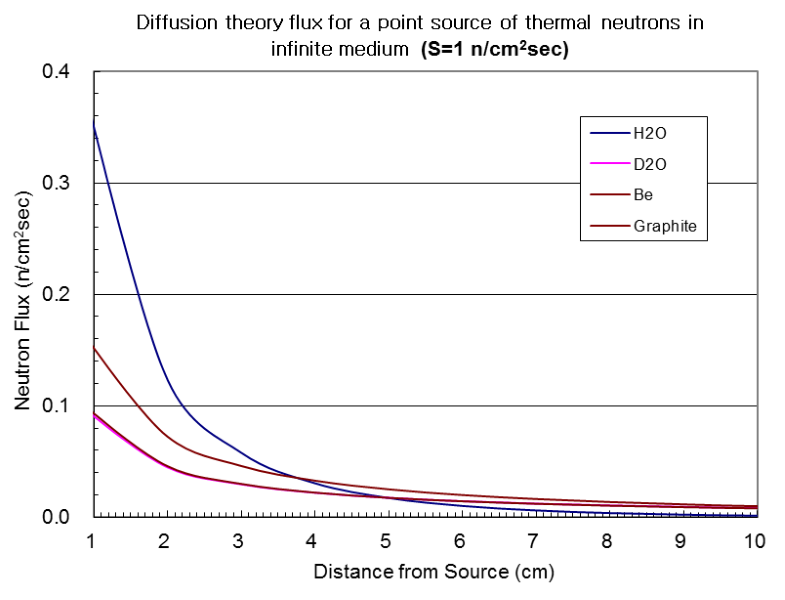
\includegraphics[width=4in]{images/dfs/dfs-shape.png}
    \caption{Flux Shape Depent On Diffusion Coefficients}\label{dfs-shape}
  \end{figure}
\item At $r=0$ tere is a non-physical singularity due to the mathematical artifact of point sources;
\item Diffusion theory is not valid near singularities;
\item We can use diffusion kernel to solve source problems in non-multiplying media by superposition.
\end{enumerate}

\clearpage
\topic{Plane Source in Infinite Non-Multiplying Medium}
The plane source is placed at $x=0$. The balance equation and the homogeneous solution are similar as the point source case except now we are in x-direction only. In a symmetric case, we can solve for one side only; for now let's consider $x>0$: 
\eqn{ \phi(x) = Ae^{x/L} + B e^{-x/L}} 
BC1: $\lim_{x \to \infty} \phi(x) = 0$ suggests that $\phi(x) = B e^{-x/L}$; BC2: $\lim_{x\to 0} J(r)  = \frac{S_0}{2}$, 
\eqn{ J = -D \dphidx = B D e^{-x/L} }
That is, 
\eqn{ \phi(x) = \frac{S_0 L}{2D} e^{-x/L}, x>0 }
For the total geometry, we can simply place an absolute sign on $x$:
\eqn{ \phi(x) = \frac{S_0 L}{2D} e^{-|x|/L}}
If the source is placed at $x=b$, the solution becomes,
\eqn{ \phi(x) = \frac{S_0 L}{2D} e^{-|x-b|/L} }


\clearpage
\topic{Plane Source in Finite Multiplying Medium with $\kinf > 1$}
For multiplying medium, we use the $B_m^2$ term instead of the $\ols$,
\eqn{ \dphidxn2 + B_m^2 \phi &= 0,  & B_m^2 &= \frac{\mu \Sigma_f - \Sigma_a}{D} = \frac{\kinf - 1}{L^2} > 0}
Assume system is subcritical with leakage, and boundary conditions are from current at center and zero flux at the H/2 boundary. Again this is a symmetric system, so we are going to solve the $x>0$ case. The homogeneous solution is,
\eqn{ \phi(x) = A \cos(B_mx) + B\sin(B_mx) }
BC1: $\phi(H/2) = 0$; BC2: $J(0) = \frac{S_0}{2}$ because of a plane source. We can solve for the coefficients,
\eqn{ \phi(x) = \frac{S_0}{2DB_m \cos\left( \frac{B_m H}{2} \right)} \sin\left[ B_m \left(\frac{H_2} - x\right) \right] }
Interpretations:
\begin{enumerate}
\item Because $\kinf > 1$, the flux shape is concave, that is, increasing negative slopes in the positive domain.  
\item If $H$ is increased to the critical dimension, that is, $H \to \frac{\pi}{B_m}$, then $\phi(0) \to \infty$; that is, if the reactor is critical, the flux at the source is infinite. That is, there is no steady-state solution for flux at the source site. In fact, if we place a fission detector at $x=0$ and measure source multiplication, 
  \eqn{M_s(0) = \frac{N_d \sigma_{f,d} V_d \phi(0)}{S_0} \propto \frac{\sigma_f}{2DB} \tan\left(\frac{BH}{2} \right) }
  Or the inverse source multiplication factor, 
  \eqn{ \frac{1}{M_s(0)} \propto \frac{1}{\tan\left(\frac{BH}{2} \right)} \to 0 }
\item To reach criticality, we can add fuel elements, withdraw control rods, and dilute boron. 
\item 1/M is useful for estimating criticality as shown in Figure~\ref{approach-critical}. Also of interest is the change of the flux shape as we increase $\kinf$. 
  \begin{figure}
    \centering
    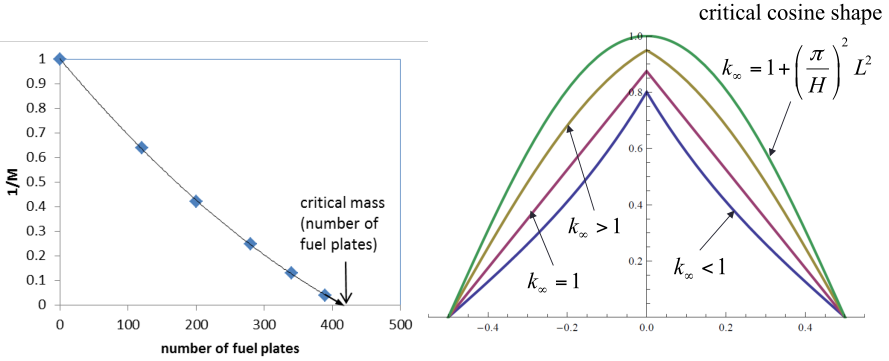
\includegraphics[width=5in]{images/dfs/approach-critical.png}
    \caption{1/M plot and Flux Shape In Approaching Criticality}\label{approach-critical}
  \end{figure}
\end{enumerate}

\clearpage
\topic{Plane Source in Finite Multiplying Medium with $\kinf < 1$}
For multiplying medium, we use the $B_m^2$ term instead of $\ols$, but for $\kinf < 1$, we know,
\eqn{ B_m^2 = \frac{\nu \Sigma_f - \Sigma_a}{D} = \frac{k_{\infty} - 1}{L^2} < 0}
For less confusion, we are going to use $-|B_m|^2$ term to replace the regular $B_m^2$ term to specify that the buckling term is negative in the case of $\kinf < 1$. Hence our balance equation is, 
\eqn{ \dphidxn2 - |B_m|^2 \phi = 0 }
The homogeneous solution is, 
\eqn{ \phi(x)  = A\cosh(|B_m|x) + B \sinh(|B_m|x) }
BCs: $\phi(0) = \phi_0, \phi(H) = 0$, we can solve for the coefficients, 
\eqn{ \phi(x) = \phi_0 \left[ \cosh(|B_m|x) - \frac{\cosh(|B_m|x)}{\sinh(|B_m|x)} \sinh(|B_m|x) \right] }
Extreme condition: if we let the size of the slab to go to infinity, 
\eqn{\lim_{H \to \infty} \phi(x) = \phi_0 [\cosh(|B_m|x) - \sinh(|B_m|x)] = \phi_0 e^{-|B_m|x} = \frac{S_0L}{2D} e^{-|B_m|x} }
Notice in both finite and infinite case, the fluxes have convex shapes; the finite curve is below the infinite curve though. 


\clearpage
\topic{Critical Finite Cube}
Consider a finite cylinder from $-H/2$ to $H/2$ with radius $R$. We assume azmimuthal symmetry of Helmholtz Equation, 
\eqn{\frac{1}{r} \ddr \left( r \pphipr\right) + \pphipzn2 + B^2 \phi = 0 }
Assume separation of variables,
\eqn{ \phi(r,z) = R(r) Z(z) }
We plut the sepration of variables into the Helmholtz Equation, break $B^2 = B_r^2 + B_z^2$, and we get two equations one for each direction, 
\eqn{ \frac{1}{R} \left( \dRdrn2 + \frac{1}{r} \dRdr \right) + B_r^2 = 0 }
\eqn{ \dZdzn2 + B_z^2 Z = 0 }
In $r$ direction, we can consider an infinite cylinder, 
\eqn{ R(r) &= A_1 J_0 (B_r r), & B_r&= \frac{2.405}{R} }
In $z$ direction, we can consider an infinite slab,
\eqn{ Z(z) &= A_2 \cos(B_z z_, & B_z &= \frac{\pi}{H} } 
We combine the two directions,
\eqn{ \phi(r,z) &= A J_0 \left( \frac{2.405}{R} r\right) \cos \left( \frac{\pi z}{H} \right), &B^2 &= B_r^2 + B_z^2 = \left( \frac{2.405}{R} \right)^2 + \left( \frac{\pi}{H} \right)^2 }
Problems with less than one direction that is non-homogeneous can be solved this way with separation of variables. 

\clearpage
\topic{Critical Finite Cylinder} 
Consider a finite cube with the dimensions $-a/2 \le x \le a/2, -b/2 \le y \le b/2, -c/2 \le z \le c/2$. The Helmholtz equation is,
\eqn{ \pphipxn2 + \pphipyn2 + \pphipzn2 + B^2 \phi = 0}
Assume separation of variables,
\eqn{ \phi(x,y,z) = X(x) Y(y) Z(z) }
Do the similar math as the finite cylinder case or by intuition, 
\eqn{ \dXdxn2 + B_x^2 X &= 0, &\dYdyn2 + B_y^2 Y &= 0, &\dZdzn2 + B_z^2 Z &=0, & B^2 &= \left(\frac{\pi}{a}\right)^2 + \left(\frac{\pi}{b}\right)^2 + \left(\frac{\pi}{c}\right)^2 }


\clearpage
\topic{Critical Reflected Slab Reactor}
Consider a critical reflected slab reactor as in Figure~\ref{reflected-slab}. 
\begin{figure}
  \centering
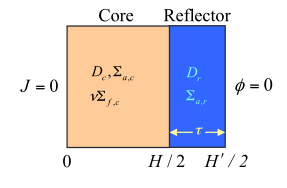
\includegraphics[width=2.5in]{images/dfs/reflected-slab.png}
\caption{A Critical Reflected Slab Geometry} \label{reflected-slab}
\end{figure}
The Helmholtz equations for the two regions are,
\eqn{-D^c \laplace \phi^c + \Sigma_a^c \phi^c &= \frac{1}{\keff} \nu \Sigma_f^c \phi^c,  &-D^r \laplace \phi^r + \Sigma_a^r \phi^r &= 0 }
If we assume,
\eqn{ B^2 &= \frac{\frac{\kinf}{\keff} - 1}{L_c^2}, & \kappa^2 &= \frac{1}{L_r^2} = \frac{\Sigma_a^r}{D^r} = -B_{m,r}^2 }
Then we are left with,
\eqn{ \laplace \phi^c + B^2 \phi^c &= 0, &\laplace \phi^r - \kappa^2 \phi^r &= 0}
The solutions are in the forms of,
\eqn{ \phi^c(x) &= C_1 \cos(Bx) + C_2 \sin(Bx), &\phi^r(x) &= C_3 \cosh(\kappa x) + C_4 \sinh (\kappa x) }
BC1: reflective boudnary condition at $x=0$,
\eqn{ J^c(0) = 0, \Rightarrow C_2 = 0}
BC2: zero flux at reflector surface, 
\eqn{ \phi(H'/2) = 0, \Rightarrow C_3 = 0} 
and interface condition: 
\eqn{ \phi^c (H/2) &= \phi^r (H/2), & J^c(H/2) &= J^r (H/2) }
which can be written in the matrix form, 
\begin{align}
\left[ \begin{array}{cc}
\cos (BH/2) & -\sinh(\kappa \tau) \\
D^c B \sin(BH/2) & -D^r \kappa \cosh(\kappa \tau) 
\end{array} \right] 
\left[ \begin{array}{c} 
C_1 \\ C_4 \end{array} \right] = 0
\end{align}
We define the reflector thickness $\tau = \frac{H' - H}{2}$, then the coefficients can be solved,
\eqn{ C_1 &= \phi^c (0), & C_4 &= C_1 \frac{\cos (BH/2)}{\sinh(\kappa \tau) } }
which gives us the criticality condition,
\eqn{ D^c B_m \tan \left(\frac{B_m H}{2} \right) = D^r \kappa \coth (\kappa \tau) }
Interpretation:
\begin{enumerate}
\item Since $B_m$ is defined with $\keff$, that is, we need to satisty an expression between $\keff$ and $H$. We can either,
  \begin{enumerate}
  \item Given $H$, search for the $\keff$ that satisfies the equivalence;
  \item Given $\keff$, search for the $H$ that satisfies the equivalence,
    \eqn{H = \frac{2}{B_m} \tan^{-1} \left[ \frac{D^r \kappa}{D^c B_m} \coth (\kappa \tau) \right] }
    That is, as $H \down, \tau \up$. For large $\tau$, like $\kappa \tau > 3, \coth (\kappa \tau) \to 1$, the smallest $H$ to reach criticality is,
    \eqn{H = \frac{2}{B_m} \tan^{-1} \left[ \frac{D^r \kappa}{D^c B_m} \right] }
  \end{enumerate}
\item Critical dimension is reduced by the presence of the reflector: 
\begin{align}
  s &= \frac{\tilde{H}}{2} - \frac{H}{2}  = \frac{\pi}{2B_m} - \frac{1}{B_m} \tan^{-1} \left[ \frac{D^r \kappa}{D^c B_m} \coth (\kappa \tau) \right] 
  = \frac{1}{B_m} \left\{ \frac{\pi}{2} - \tan^{-1} \left[ \frac{D^r \kappa}{D^c B_m} \coth(\kappa \tau) \right] \right\} \\
  \tan\left[ \frac{\pi}{2} - \tan^{-1} x \right] &= \cot [\tan^{-1} x ] = \frac{1}{\tan[\tan^{-1} x]} = \frac{1}{x} \\
  \frac{\pi}{2} - \tan^{-1} x &= tan^{-1} \left( \frac{1}{x} \right) \\
  s &= \frac{1}{B_m} \tan^{-1} \left[ \frac{D^c B_m}{D^r \kappa} \tanh(\kappa \tau) \right] 
\end{align}
For larger cores, $B_m \to 0$ and $\tan^{-1} x \approx $, that is, 
\eqn{ s = \frac{D^c}{D^r \kappa} \tanh(\kappa \tau) = \frac{D^c}{D^r} L^r \tanh\left( \frac{\tau}{L^r} \right) }
That is, 
\begin{align}
  \left\{ \begin{array}{cc} 
    \tau \ll L^r & s \approx \frac{D^c}{D^r} \tau, (\tanh x \approx x \mbox{ for }x\ll 1) \\
    \tau \gg L^r & s \approx \frac{D^c}{D^r} L^r, (\tanh x \approx 1 \mbox{ for }x > 3) 
  \end{array} \right. 
\end{align}
\end{enumerate}


\clearpage
\topic{Summary}
\begin{enumerate}
\item \textit{Super-positioning of sources}: if we are given a random source that is the sum of a couple of common forms of sources, we can super-position the flux from each of the common sources. This method works in any non-multiplying medium, and in multiplying medium in subcritical condition\footnote{Supercritical condition, as source increaes, flux inverts}. For instance, we can super-position point sources to get a line source. 
\item Diffusion theory is not valid near singularities. 
\item $\kinf$ is important\footnote{know this for the exams}: 
  \begin{enumerate}
  \item $\kinf = 1$: flux is straight line;
  \item $\kinf < 1$ means $B^2 < 1$, flux is $\sinh, \cosh$ which is convex; 
  \item $\kinf > 1$ means $B^2 > 0$, flux is $\sin, \cos$ which is concave. 
  \end{enumerate}
\item Know how to get the critical buckling for different geometries. 
\item Seperation of variables works as long as there is no one more than one direction that is heterogeneous. 
\end{enumerate}

  \begin{table}
    \centering
    \begin{tabular}{|c|c|c|c|} \hline
      Source & Geometry & BC2 & Flux \\ \hline \hline
      Point & Infinite Sphere &$\lim_{r\to 0} 4 \pi r^2 J(r) = S_0$ & $\frac{S_0}{4\pi D} \frac{e^{-r/L}}{r}$ \\ \hline
      Plane & Infinite Slab & $\lim_{x\to 0} J(r)  = \frac{S_0}{2}$ & $\frac{S_0 L}{2D} e^{-|x|/L}$ \\ \hline
    \end{tabular}
    \caption{Subcritical System: Source and Flux} 
  \end{table}
  
  
\end{document}
